\documentclass[10pt,conference,compsocconf,a4paper]{IEEEtran}
% \documentclass[10pt,a4paper]{IEEEtran}

\usepackage{graphicx}
\usepackage{amsmath, amssymb}
\usepackage{commath}
\usepackage{booktabs}
\usepackage{siunitx}
\usepackage[labelformat=simple, labelfont=normalfont]{subcaption}  % Side-by-side figures
% \usepackage[labelfont=sc]{caption}  % Using captionof outside of figure environment
\usepackage[colorlinks, bookmarks=false, citecolor=black, linkcolor=black, urlcolor=blue]{hyperref}  % Cite colors + autoref
\usepackage{xurl}  % hypen breaks in urls

\newcommand{\G}{\mathcal{G}}
\renewcommand{\vec}[1]{\boldsymbol{#1}}
\newcommand{\funit}[1]{\ [\si{#1}]}  % formula unit
\newcommand{\nunit}[1]{\ \si{#1}}  % numerical unit
\newcommand{\avg}[1]{\langle{#1}\rangle}

% braces around equation number in referencing
\makeatletter
\let\oldtheequation\theequation
\renewcommand\tagform@[1]{\maketag@@@{\ignorespaces#1\unskip\@@italiccorr}}
\renewcommand\theequation{(\oldtheequation)}
\makeatother

% Prevent latex from streching out paragraph spacings
\raggedbottom

% braces around subfig number
\renewcommand\thesubfigure{\,(\alph{subfigure})}

% Smallcaps short autoref
\newcommand*{\shortautoref}[1]{%
	\begingroup
	\def\equationautorefname{\textsc{Eq.}}%
	\def\tableautorefname{\textsc{Tab.}}%
	\def\figureautorefname{\textsc{Fig.}}%
	\autoref{#1}%
	\endgroup
}

% Itemize spacing
\let\olditemize=\itemize
\let\endolditemize=\enditemize
\renewenvironment{itemize}{\olditemize \itemsep0em}{\endolditemize}

% subfigure spacing
% \captionsetup[subfigure]{aboveskip=1pt}

\begin{document}
\title{Convolutional graph neural networks for tracking budding yeast cells in timelapse microscopy}

\author{
	N. Vadot, F. Massard, G. Brenna, S. Rahi, V. Gligorovski
}

\maketitle

\begin{abstract}
	In many bioimaging applications, segmentation algorithms are used in order to treat microscopy images.
	% This is nowadays done using deep learning methods, which achieve human-like performance and accelerate research.
	However time-lapse microscopy, an additional requirement is to identify same cells on different snapshots, a problem known as tracking.
	% However, one often overlooked problem is that of tracking cell masks throughout movies.
	This post-segmentation step is often done using classical bipartite graph matching algorithms.
	% (e.g. Hungarian algorithm, as implemented in YeaZ \cite{dietler_convolutional_2020})
	Often manual labor is required to double-check cell masks are tracked correctly throughout the movie. This is especially time-consuming for large cell colonies or long movies, and the performance of classical algorithms degrades quickly as the time difference between images grows.
	We present a cell mask tracking method based on recent advancements in deep graph convolutional networks \cite{li_deepergcn_2020}. This method achieves better accuracy than classical algorithms, thanks to the context-awareness of the graph structure. Our method (1.) extracts simple geometrical information from a dataset of budding yeast masks, 
	% (2.) translates the tracking problem to a binary classification problem,
	(2.) feeds the extracted information into a graph convolutional neural network, 
	(3.) applies linear cost optimizations to the output scores of the neural network, producing 
	(4.) an assignment matrix which directly translates back to cell mask trackings.
	% For this, we train on a dataset of segmented budding yeast images, containing 5 colonies each growing to approximately 110 cells by the end of the 180 frames.
	% Since this method works directly on cell masks, it is agnostic of the specific segmentation algorithm used, and should generalize well to any other mask tracking problem involving circular cells.
	Cutting down on manual labor, this method performs with near-perfect accuracy on hard tracking problems, even in when cells crowd or move from their place of birth.
\end{abstract}


\section{Introduction and problem statement}

	The tracking problem emerges in timelapse microscopy, where images of a cell colonies are taken at a fixed rate (typically around one image every 5 to 15 minutes for budding yeast). Segmentation of these images refers to finding the pixelwise masks that cover each cell visible in a given image. Each cell is then given a unique identifier, and tracking translates to matching each cell of the current image to a cell in the next image. This is a particularly challenging task for fast-growing microbes, such a budding yeast. Dependingly on the time interval between each image, the cell colony might have changed significatively: new buds appear, cell geometry changes due to growth or pressure from neighbouring cells, cells get flushed away or move around.

	Correct tracking of cells is especially important when addressing a more specific problem, that of lineage determination of budding yeast: for each new bud, the parent cell needs to be determined. This is made difficult in densely packed environments. One solution to this problem is the use of fluorescent markers that label the site of emerging bud on the parent cell. However, it might not always be convenient to use such markers, in which case one can only rely on the microscopy images and the corresponding segmentations. If mistakes are made during tracking of the cell masks, then this directly causes mistakes in the lineage relationships, which utilize the same cell identifiers as the masks.
	
	% and the question arises if lineage determination is possible with only a phase contrast image. Buds are most visible when they grow, so a machine learning algorithm might be able to pick up on spatio-temporal correlations in the segmentations to determine the parent. However, feeding a machine learning algorithm coherent temporal information requires a consistent tracking of the cells, which is the main problem this report addresses.

	The classical approach to tracking is to extract features such as mask position and size from the segmentation geometry, % (YeaZ uses cell surface area and center of mass),
	and minimize the pairwise Euclidean distance in the feature space using a bipartite matching algorithm. The problem with this method is that it starts to break down for large colonies, since in that regime many cells have similar geometry or start drifting away from the colony.
	
	The key observation based on which we built our method is that cells not only have features (area, radius, eccentricity, etc.) of their own, but also exist in a neighborhood of other cells. In other words, a lot of identifying information is encoded in the \textit{neighbourhood} of each cell, such as the relative position with each neighbour, and the features of neighbouring cells.

	% Then, it would be interesting to look at pairwise relationships between cells and their nearest neighbors to track the cells, similarly to how puzzle pieces fall into place given the right context.

	A graph is the most intuitive way to store this information, where cells are represented by nodes, and edges link nearest neighbours together. Nodes then store cell features, and edges store relative positions of a cell pair. This graph representation is especially powerful, as it directly encodes locality in the colony, and repeatedly performing graph convolutions lets this information diffuse to neighbouring cells.
	% A graph-based approach arises, which can naturally encode cells as nodes with certain features, and nearest-neighbor relationships are edge features.
	The recent development of graph neural networks (GNN) \cite{zhou_graph_2021} and growing open-source codebase \cite{paszke_pytorch_2019, fey_fast_2019} makes these methods attractive for solving the problem of tracking cells in a timelapse microscopy.

\section{Prior work}
	
	Most of the state-of-the-art cell tracking methods rely on conventional algorithms such as bipartite matching \cite{bipartite, dietler_convolutional_2020} and Viterbi \cite{viterbi, viterbi2}. Bipartite matching (also equivalently found under the names of ``assignment problem'', ``linear cost optimization'' or ``Hungarian algorithm'') assigns a cost to each possible pair of cell matching between the current and next image. For instance in YeaZ \cite{dietler_convolutional_2020}, this cost is derived from the Euclidean distance in feature space (center of mass and area) between a pair of cells. The Viterbi algorithm models the change of individual cell features as a Markov process, and maximizes the likelihood of the hidden intermediate cell features resulting in the observed features on the next frame.
	
	However, these traditional approaches have limitations and deep learning methods have proven to have great potential to improve performance. In recent years, various Convolutional Neural Networks (CNN), and recurrent CNN-based approaches have been introduced for tracking cells in microscopy images (e.g. \cite{he,delta,payer,hayashida,moen}).

    While they have proven useful for general cell tracking tasks, currently available tracking tools designed specifically for budding yeast imaging still often rely on traditional approaches. Nevertheless, new methods are being developped, based for instance on a Fourier transform of cell neighbourhoods in microscopy images \cite{Cuny2022}.
	Tracking is particularity challenging since budding yeast cells bud approximately every 90 minutes, grow fast, and tend to drift away under the influence of growth media flow.
	% This is due to the particularity of budding yeast, where cells bud frequenty (the cell-cycle time of budding yeast is around 90 minutes), grow fast, move around the colony, and microscopy images are sparse in time. 
	% a robust deep learning-based cell tracker for yeast cells has not been proposed yet.
	Recent works on segmentation and tracking of budding yeast cells in brightfield microscopy focus rather on developing and training networks for segmentation, than on updating tracking techniques that are still based on conventional algorithms \cite{dietler_convolutional_2020,yeastnet,kruitbosch}.

    This paper proposes a novel graph neural network (GNN) approach for tracking yeast cells from segmentations. 
	We take inspiration from tracking algorithms used in particle trajectory reconstruction in detectors \cite{dezoort_charged_2021}, where geometrical features of detection events are encoded using a simple Multi-Layer Perceptron (MLP), after which a classifier attributes multiple detection events to the same particle. We also apply ideas from \cite{kipf_semi-supervised_2017}, which considers the problem of finding a subgraph in a larger graph. It does so by applying graph convolutions, embedding the nodes in a high-dimensional space, and minimizing the total cost of pairwise Euclidean distance to match nodes from the two graphs.
	We thus reformulate the tracking problem as a graph matching problem, and use a similar idea by maximizing a score to assign nodes between two graphs.

	% It takes inspiration from tracking algorithms used in particle trajectory reconstruction in detectors \cite{dezoort_charged_2021}.
	% In this approach, timestamped detection events in cylindrical coordinates are represented as nodes, and edge features are constructed by considering geometrical differences of the two detection events it connects. Features are then encoded with an MLP, and an edge-classification task is performed in order to attribute multiple detection events to the same particle. In our context, cells are not moving in a highly correlated manner like a particle through a detector, but the idea of encoding geometrical features can be repurposed.

	% Tracking nodes, as they evolve in time-dependent graphs, can be thus be reformulated as the problem of graph matching. \cite{kipf_semi-supervised_2017} considers the problem of finding a subgraph in a larger graph. It does this by applying graph convolutions, embedding the nodes in a high-dimensional space, and minimizing the total cost of pairwise Euclidean distance to match nodes from the two graphs. We try to reformulate the tracking problem as a graph matching problem, and use a similar idea by maximizing a score to assign nodes between two graphs.

	% Other papers \cite{cordonnier_extrapolating_2019} propose a graph neural network-based approach to predict trajectories, however they assume highly correlated motion or decision agents responsible for the motion, which is not applicable here. Furthermore, the task here is to reconstruct trajectories, not to predict them.

\section{Data preprocessing} \label{sec:data_preprocessing}

	\subsection{Feature extraction and cell graph generation} \label{sec:data_preprocessing:featext}

		The full data preprocessing pipeline is schematized in \shortautoref{fig:pipeline}. The data used here consists of 5 colonies of budding yeast, with microscopy images taken at 5 minute intervals, for a total of 180 images (15 hours of growth time) per colony. On average, the colonies started with approximately 2 cells and had around 110 cells at the end.

		% NOTE: removed since we already mentioned the train/val datasplit in section V
		% The first 4 colonies (in the data, named \texttt{colony00[0123]}) are used for generating training (and validation) datasets, and the last colony (named \texttt{colony007}) is kept as a final testing set.

		To generate the ground truth dataset, the movies were segmented and manually tracked using YeaZ \cite{dietler_convolutional_2020}. From the segmentation masks, simple geometrical features were extracted from the cells: mask surface area $A$, radius $r$ and eccentricity $e$. To do this, an ellipse was fitted to the cell by using PCA analysis on the cell mask coordinates, which can then be used to obtain the semi-major and minor axes $a$ and $b$ respectively. Then we compute $e=\sqrt{1-(\frac{a}{b})^2}$, and the radius of the circle with the same area as the ellipse $r=\sqrt{ab}$. \shortautoref{fig:hist_x} shows the distribution of the node features. The distributions are strongly peaked around their mean, respectively $\avg{A} \approx 21 \pm 14 \nunit{\micro \meter \squared}$, $\avg{r} \approx 2.5 \pm 0.8 \nunit{\micro \meter}$ and $\avg{e} \approx 0.52 \pm 0.14$. Notice the distribution for $r$ has a few outliers corresponding to very large cells, and these outliers are even more visible for $A$, explained by the scaling law $A \sim r^2$.
		% It however doesn't make sense to remove these outliers, since that would have the same effect as removing the cell from the colony, impacting its direct neighbors.

		To extract nearest neighbour features, we first extracted the contour of each cell mask. Cells are considered neighbours if the minimal distance between their contours is below $1.3 \nunit{\micro \meter}$ (about half a mean cell radius), which is a parameter that can be adjusted.
		% (this threshold is arbitrary, and can be changed as needed when calling \texttt{bread\_nn.graph.build\_cellgraph}).\
		Extracted features are $\rho$, the center of mass (CM)-to-CM distance between the neighboring cells, $\theta$, the angle of the CM-to-CM vector with respect to the horizontal axis, and $\ell$, the minimal distance between the contours. \shortautoref{fig:hist_e} shows the distribution of these features. $\rho$ shows a distribution peaked around $\avg{\rho} \approx 5.4 \pm 1.2$, which is in accordance with the average cell radius of $r \approx 2.5 \nunit{\micro \meter}$ meaning two average cells would be separated by approximately $2r \approx 5.0 \nunit{\micro \meter}$. $\theta$ shows a near-uniform distribution, with mean and standard deviation $\avg{\theta} \approx 0 \pm 1.8$. Again, this is intuitive, since we don't expect cells to be preferentially aligned in one direction. Note that we allow $\theta$ to take values in $[-\pi, \pi]$ instead of $[0, \pi]$, because edges are not stored bidirectionally (to save memory), so the sign of $\theta$ encodes directionality of the edge. $\ell$ is strongly peaked around $\avg{\ell} \approx 0.34 \pm 0.22 \nunit{\micro \meter}$. Physically, $\ell$ is not an exact representation since cell edges are supposed to be in contact, and the mean being slightly offset is an artifact from the segmentation process.
		% \footnote{
		This artifact is a result from the watershed algorithm used to segment the output of YeaZ's CNN. The connectivity parameter is set to a nonzero value, resulting in gaps between neighouring cell masks.
		% }
		Nevertheless, $\ell$ can be a good distance metric between cells, since it is independent of their sizes.

		% In total, 5 colonies $\times$ 180 images = 900 cell graphs are constructed.
		% (note: edges are considered bidirectional, but are stored as one-directional to save memory). The Python notebook used for this process can be found under \texttt{experiment\_gnn/build\_cellgraphs.ipynb}.

		\begin{figure}
			\centering
			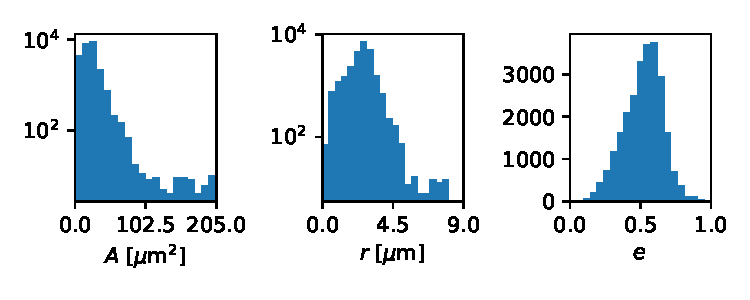
\includegraphics[width=\linewidth]{figures/hist_x.pdf}
			\captionof{figure}{Histogram of node features (20 bins). For area and cell radius, a log scale is used in order to emphasize the outliers (very large cells). Sample size is 25510 nodes.}
			\label{fig:hist_x}
		\end{figure}
	
		\begin{figure}
			\centering
			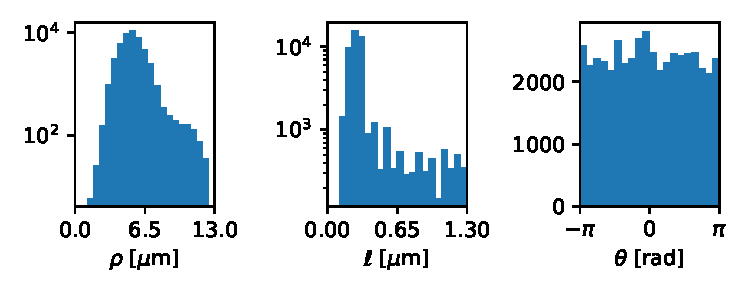
\includegraphics[width=\linewidth]{figures/hist_e.pdf}
			\captionof{figure}{Histogram of edge features (20 bins). For CM-to-CM and cell contour distance, a log scale is used. Sample size is 48018 edges.}
			\label{fig:hist_e}
		\end{figure}

	\subsection{Assignment graph generation}

		% We formulate the tracking problem as a graph matching problem.
		Suppose we have generated two graphs $\G^{(1)}$ and $\G^{(2)}$ storing extracted features from two segmentations. The goal is to track cells from $\G^{(1)}$ to $\G^{(2)}$, that is to match the nodes $\vec{v_i^{(1)}}$ of the first graph to nodes $\vec{v_a^{(2)}}$ of the second graph. An edge $\vec{e_{i,j}^{(1)}}$ is placed between nodes of the first graph if cells $i$ and $j$ are neighbours, and edges of the second graph $\vec{e_{a,b}^{(2)}}$ are constructed similarly. We store features obtained as explained in \shortautoref{sec:data_preprocessing:featext} in the respective nodes and edges.
		
		The tracking problem is converted to a binary classification problem by constructing an assignment graph $\G^{(a;x,e)}$, composed of nodes $\vec{v_{ia}^{(a)}}$ and edges $\vec{e_{ia,jb}^{(a)}}$.
		Nodes $\vec{v_{ia}^{(a)}}$ are obtained by concatenating features from $\vec{v_i^{(1)}}$ and $\vec{v_a^{(2)}}$. Edges $\vec{e_{ia,jb}^{(a)}}$ of $\G^{(a)}$ link nodes $\vec{v_{ia}^{(a)}}$ and $\vec{v_{jb}^{(a)}}$ if $\vec{e_{i,j}^{(1)}}$ and $\vec{e_{a,b}^{(2)}}$ exist in $\G^{(1)}$ and $\G^{(2)}$ respectively (i.e. cells $i,j$ are neighbours, and $a,b$ are neighbours), in which case the corresponding edge features are concatenated.

		Finally, we construct the corresponding target graph $\G^{(a;y)}$ in a similar manner, where the node features are 2-dimensional one-hot encoded vectors, indicating whether a node $\vec{v_{ia}^{(a)}}$ corresponds to a correct tracking. In other words, we want to have $1$ if the tracking $i \rightarrow a$ is correct, and $0$ otherwise. Note that at this point, there is no trace left of the cell ids that were used to differentiate cells in the segmentations.

		Assignment graphs $\G^{(a;x,e)}$ and $\G^{(a;y)}$ then correspond to the GNN input and training target respectively.
		To create the dataset used for training, we take one frame of the movie, and generate assignment graphs with each of the (up to) 20 following frames. This is repeated for every frame in every colony, creating a dataset of 8550 assignment graphs.
		% we loop over all pairs of segmentations separated by at most 20 frames (1h40), constructing the input and target assignment graphs for each pair, and repeat this for each colony.
		% The Python notebook used for this process can be found under \texttt{experiment\_gnn/build\_assgraphs.ipynb}.

		\begin{figure*}
			\centering
			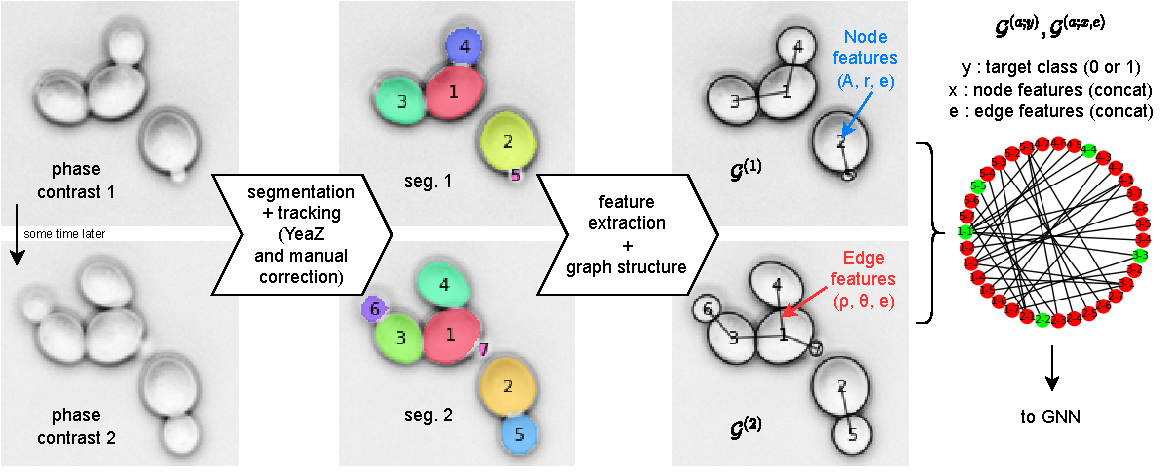
\includegraphics[width=\linewidth]{figures/pipeline.v2.pdf}
			\caption{Data preprocessing pipeline. A phase contrast timelapse microscopy of a budding yeast colony is taken, then YeaZ \cite{dietler_convolutional_2020} is used to segment individual frames, and semi-automatically track cells. Manual corrections to segmentation and tracking are applied as required. From the segmentations, geometric features are extracted, as well as features describing the neighborhood of each cell. This is stored in a graph structure $\G^{(1)}$ and $\G^{(2)}$, from which an assignment graph $\G^{(a;x,e)}$ is built. A ground truth assignment graph $\G^{(a;y)}$ is also built. Both assignment graphs are then used by the GNN for training.}
			\label{fig:pipeline}
		\end{figure*}


\section{Methods}

	\subsection{GNN structure}

		The GNN structure is summarized in \shortautoref{fig:nn}. Node and edge features of $\G^{(a;x,e)}$ are embedded by two MLPs with ReLU activation. The resulting embedded graph is then convolved by multiple DeepGCN layers \cite{li_deepergcn_2020}. One DeepGCN layer consists of a batch normalization layer (LayerNorm), an activation function (ReLU), one dropout layer, one GENConv layer, then finally a residual connection layer. In particular, the GENConv layer constructs messages $\vec{x_i}'$ from node and edge features $\vec{x_i}, \vec{e_{i,j}}$ as
		$$
			\vec{x_i}' = \textrm{MLP}(\vec{x_i}' + \sigma(\{\textrm{ReLU}(\vec{x_i} + \vec{e_{i,j}}) + \epsilon \;|\; i \in \mathcal{N}(j)\})),
		$$
		where $\mathcal{N}(j)$ denotes indices of the nodes connected to node $j$, $\sigma$ is the softmax function, and $\epsilon$ is a small learnable constant. The $\textrm{MLP}$ has 2 layers, and preserves the number of channels of the input.

		The final linear layer maps the embedded node channels to two channels, and the resulting graph $\G^{(a;\hat y)}$ is then passed to CrossEntropyLoss along with the ground truth $\G^{(a;y)}$ for backpropagation.

	\subsection{Making predictions} \label{sec:methods:pred}

		Let $n_1$ and $n_2$ be the number of cells in the first and second image, respectively. We define an assignment matrix $A$ with components $A_{i,a} = 1$ if cell $i$ in the first image is the same as cell $a$ in the second image, else $A_{i,a} = 0$. For the example in \shortautoref{fig:pipeline}, the assignment matrix is
		$$
			A = \begin{pmatrix}
				1 & 0 & 0 & 0 & 0 & 0 & 0 \\
				0 & 1 & 0 & 0 & 0 & 0 & 0 \\
				0 & 0 & 1 & 0 & 0 & 0 & 0 \\
				0 & 0 & 0 & 1 & 0 & 0 & 0 \\
				0 & 0 & 0 & 0 & 1 & 0 & 0
			\end{pmatrix}.
		$$
		Notice the last two columns are zero, corresponding to the fact the cells \#6 and \#7 are buds that consequently do not appear in the first image.

		The predicted graph $\G^{(a;\hat y)}$ contains edges $\vec{\hat y}_{i,a} = (Z_{i,a,0}, Z_{i,a,1})$. In artificial neural network terminology, $Z_{i,a,0}, Z_{i,a,1}$ are often called ``drive'' or ``potential'', since they enter the softmax function, and yield a classification probability between 0 and 1.\footnote{Note : the case of 2-class cross-entropy loss (softmax, followed by negative-log-likelihood loss (NLLL)) used here reduces to binary classification (sigmoid, followed by NLLL), where the corresponding sigmoid activation function $\sigma(a)$ drive is $a = Z_{i,a,0} - Z_{i,a,1}$. Both approaches are equivalent.}
		From the predicted graph $\G^{(a;\hat y)}$, we can therefore construct an assignment matrix by reshaping the node features into a matrix $Z$ of shape ($n_1$, $n_2$, $2$), where the last dimension stores weights for the classification decision.
		In other words, $Z_{i,a}$ stores the two classification weights of the tracking $i \rightarrow a$. By taking differences along the last axis of $Z$, we obtain a score matrix $S$ of shape ($n_1$, $n_2$). If $S_{i,a} = Z_{i,a,0} - Z_{i,a,1} > 0$, the classification weight for "yes" is larger than for "no", and vice-versa. The magnitude of $S_{i,a}$ can therefore be interpreted as the GNN's confidence of the classification.

		To transform $S$ into $A$, the simplest approach might be to assign $A_{i,a} = 1$ if $S_{i,a} > 0$, and $A_{i,a} = 0$ otherwise. However, this can lead to situations where a cell in the first frame gets tracked to multiple cells of the second frame. Another approach might be to maximize $S$ row-wise, in which case we ignore the fact cells can be flushed away between two frames. Maximizing $S$ column-wise, we run into the problem that multiple cells of the first frame can get tracked to one cell of the second frame. Instead, we want to maximize the total score over all possible matchings, mathematically we find $A^\star$ which verifies
		$$
			A^\star = \arg \max_{A \in \{0, 1\}^{n_1 \times n_2}} \sum_{i,a} S_{i,a} A_{i,a}.
		$$
		This is a linear sum assignment, which can be solved using \texttt{scipy.optimize.linear\_sum\_assignment} from the Scipy package \cite{2020SciPy-NMeth}.

		For the following, we denote the predicted assignment matrix by $\hat A := A^\star$.

		% There are multiple ways of transforming $Z$ into $A$, but we describe only the method that empirically worked the best (other methods are presented and discussed in \texttt{experiment\_gnn/pipeline.ipynb}).

		% By taking differences along the last axis of $Z$, we obtain a score matrix $S$ of shape ($n_1$, $n_2$), where each entry's magnitude can be interpreted as the confidence of the GNN of the assignment.

		% The goal is then to find $A^\star$ as such to maximize the assignment score, mathematically
		% $$
		% 	A^\star = \arg \max_{A \in \{0, 1\}^{n_1 \times n_2}} \sum_{i,a} S_{i,a} A_{i,a}.
		% $$
		% This linear sum assignment (linsum) is easily solved by using \texttt{scipy.optimize.linear\_sum\_assignment} from the Scipy package \cite{2020SciPy-NMeth}.

		\begin{figure*}
			\centering
			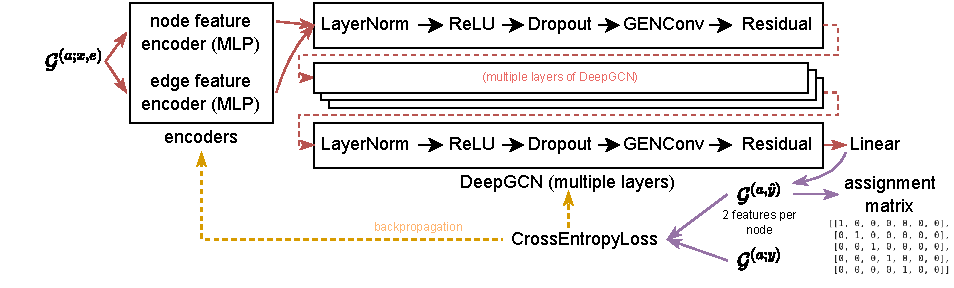
\includegraphics[width=\linewidth]{figures/nn.v2.pdf}
			\caption{The GNN structure. For a given input graph, the node and edge features are encoded by MLPs. The resulting graph is then convolved multiple times following DeepGCN \cite{li_deepergcn_2020}. A final linear layer maps the encoded node features down to two, and CrossEntropyLoss is computed for backpropagation. For evaluation, the node features of $\G^{(a;\hat y)}$ can be reduced and reshaped to build an assignment matrix.}
			\label{fig:nn}
		\end{figure*}


\section{Results}

	This section discusses performance on the models trained with the constructed graphs, as described in \shortautoref{sec:data_preprocessing}. All models are trained with the Adam optimizer with varible exponentially decaying learning rate, adjusted manually depending on the batch size used. Unless specified otherwise, all layers use dropout (if it applies) during training with probability parameter $0.1$. The random seed is fixed at the start of each training session. The dataset is split into training and validation subsets with respective ratios of $80\%$ and $20\%$, and the training dataset is reshuffled at each epoch.

	For evaluation, the assignment matrix predicted by the model, $\hat A$ is compared to the ground truth $A$ using the following accuracy metric:
	$$
		\textrm{acc}(\hat A, A) = \frac{1}{n_1 n_2} \sum_{i,j} \delta_{A_{i,j}, \hat{A}_{i,j}}.
	$$

	\subsection{MLP baseline}

		To assess whether the graph structure is actually informative for the tracking task, we train a MLP on the node features $\vec{X}$ of $G^{(a;x,e)}$. This task can be thought of as taking two cells from two different frames, and asking whether they are the same.

		% As a baseline for the GNN, we train a MLP on the node features $\vec{X}$ of $G^{(a;x,e)}$ to evaluate if the graph structure (that is, addition of edge features) really adds valuable information for learning.

		In order to not bias the MLP during training, we need to equilibrate the labels $\vec{y}$, because the number of nodes in the assignment graph grows as $n_1 n_2$, but the number of assignments where $y=1$ grows as $n_1$. Therefore, labels $y=1$ are underrepresented in large graphs, and equilibration is done by randomly removing samples where $y=0$ from the training batch, until both classes are equally represented.

		Furthermore, batch normalization is applied before the MLP in order to improve training, as described in \cite{ioffe_batch_2015}.

		A hyperparameter scan was performed on the number of MLP layers and hidden channels, and found that the best performing MLP obtained an accuracy of approximately $0.88$. More layers and hidden channels were found to marginally improve the accuracy, before it started to drop due to overfitting (data not shown).

	\subsection{GNN performance}

		\paragraph*{Hyperparameter analysis} We perform a scan on the following hyperparameters: $N_\textrm{enc}$ number of layers in both encoder MLPs, $N_\textrm{conv}$ number of DeepGCN layers, and $N_\textrm{dim}$ the number of hidden channels. Other hyperparameters, such as dropout, learning rate, exponential learning rate decay and training batch size were found to not significatively improve final performance, but can decrease training time if correctly chosen (here they were set to $0.1$, $\sim 10^{-4}$, $\sim 0.98$, $\sim 32$ respectively). For the study, we chose $N_\textrm{enc} \in \{1,2,3,4,5\}$, $N_\textrm{conv} \in \{1,2,3,4,5,8,11\}$ and $N_\textrm{dim} \in \{30, 60, 90, 120\}$. \shortautoref{fig:hparams} plots the results of the hyperparameter scan in parallel coordinates.

		\begin{figure}
			\centering
			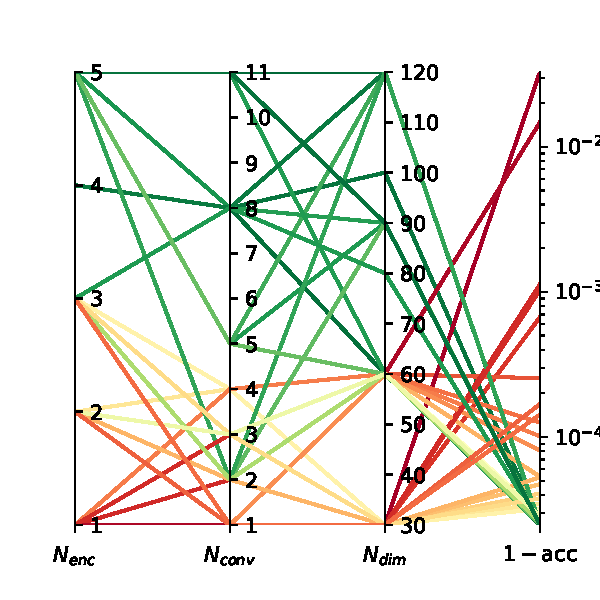
\includegraphics[width=\linewidth]{figures/hparams.pdf}
			\caption{Parallel coordinates plot of the hyperparameter scan. The best performing model uses $N_\textrm{enc}=5$, $N_\textrm{conv}=11$, $N_\textrm{dim}=120$, but a very similar performance can be achieved for less parameters, $N_\textrm{enc} \geq 3$, $N_\textrm{conv} \geq 8$ and $N_\textrm{dim} \geq 80$.}
			\label{fig:hparams}
		\end{figure}

		Models with less than $0.99$ mean accuracy are obtained with few parameters overall, $N_\textrm{enc} \in \{1,2,3\}$, $N_\textrm{conv} \in \{1,2,3,4\}$ and $N_\textrm{dim} \in \{30, 60\}$. For better accuracy, it was found most effective to increase the number of encoder layers $N_\textrm{enc} \in \{2,3\}$, which systematically drove up the mean accuracy up to $0.999$. Following this, increasing $N_\textrm{enc}$ only marginally improved accuracy, but allowing up to 5 convolution layers gave models obtaining mean accuracy of up to $0.9999$. In this regime, the graph neural network is able to capture most of the complexity of the problem, but still struggles with edge cases (for instance, a cell moving by a large amount). Further increasing the number of parameters (via $N_\textrm{conv}$ or $N_\textrm{dim}$, they seem to compensate each other) results in even better accuracy, where edge cases are now correctly handled. The best models obtained a mean accuracy of $0.99997$, and utilized $N_\textrm{enc} \geq 3$, $N_\textrm{conv} \geq 8$ and $N_\textrm{dim} \geq 80$.

		\paragraph*{Biological intuition on the role of $N_\text{conv}$ and $N_\text{enc}$} Intuitively, the performance gain of increasing $N_\textrm{enc}$ eventually caps off, because each cell graph node or edge is decribed with only 3 features, and the MLP can only transform information it is given. One way of understanding the role of increasing $N_\textrm{conv}$, is by observing one convolution can exchange information between nodes separated by one edge, and further convolutions diffuse that information to further neighbors, such that increasing the number of convolutions effectively increases the  ``communication distance'' between cells, meaning each node has a ``better view'' of the whole graph structure. This of course comes with the cost of requiring more dimensions to store the information in, explaining the need to increase $N_\textrm{dim}$, and how both compensate each other. It is not useful to be able to ``see'' further in the graph ($N_\textrm{conv}$ large) if you cannot ``store'' the information ($N_\textrm{dim}$ small), and vice-versa.

		\paragraph*{Comparison to Hungarian algorithm} We now compare the performance of the best GNN model ($N_\textrm{enc}=5$, $N_\textrm{conv}=11$, $N_\textrm{dim}=120$) against a classical Hungarian algorithm. For this, we use YeaZ's integrated tracking algorithm, which uses cell area and position, then computes the weighted pairwise euclidian distance between cell features, giving three times more weight to cell position than area. The pairwise distances are then used as costs in the Hungarian algorithm.

		We use the test dataset on time differences of up to 45 minutes (half the cell cycle period of budding yeast), and compute the accuracy of the Hungarian algorithm and our tracking method.
		A strip-plot of the accuracies as function of time difference $\Delta t$ is shown in \shortautoref{fig:timediff_accuracy} a), and one can see that the distribution of accuracies for a given $\Delta t$ is strongly peaked at $\text{acc}=1$, rendering a mean accuracy metric uninsightful (nevertheless, it is plotted for transparency in \shortautoref{fig:mean_acc}). A metric more robust to outliers is to compute the number of trackings with $\text{acc} = 1$, and normalize it by the number of trackings for a given $\Delta t$. This is plotted in \shortautoref{fig:timediff_accuracy} b), and shows our method outperforms the Hungarian algorithm for all time differences, and its performance decays more slowly as the frames become increasingly spaced in time. The graph structure therefore provides valuable information for tracking, especially in situations where images are taken infrequently.

		% After a 30 minute time difference, our method however starts decaying faster. This is probably due to the emergence of new buds: since the cell cycle of budding yeast is around 90 minut

		\begin{figure}
			\centering
			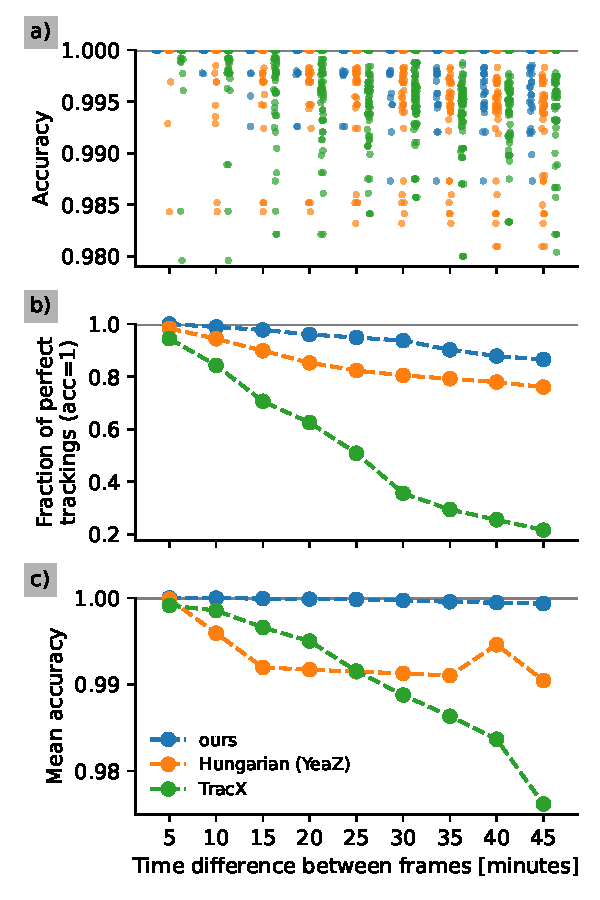
\includegraphics[width=\linewidth]{figures/timediff_accuracy.pdf}
			\caption{a) Accuracy strip-plot and b) fraction of perfect trackings as a function of time difference between frames. A perfect tracking is defined as a prediction containing no tracking mistakes. Note that this plot omits some accuracy outliers around 0.3, originating from the Hungarian algorithm. At the minimal time difference of 5 minutes, the Hungarian algorithm makes 3 mistakes (see \shortautoref{fig:mistracks}), whereas our method makes none. The performance decays as time between frames increases, and the tracking task becomes harder. The Hungarian algorithm's accuracy decays much faster than the GNN, showing our method is more stable, as well a performing better.}
			\label{fig:timediff_accuracy}
		\end{figure}

		\begin{figure}[h!]
			\centering
			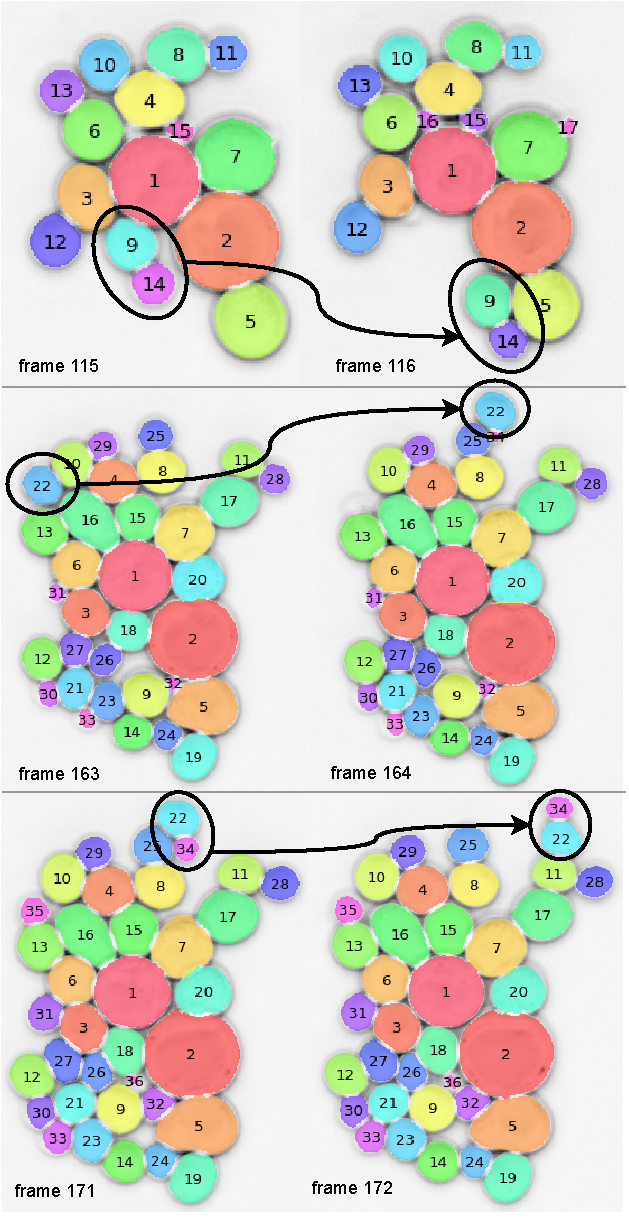
\includegraphics[width=\linewidth]{figures/mistracks.pdf}
			\caption{Segmentations from the test dataset highlighting moving cells. Out of the 179 interframes, YeaZ makes 3 tracking mistakes. On frame 115, cells 9 and 14 move together towards cell 5, and YeaZ tracks cell 9 to cell 16 and cell 14 to cell 9. On frame 163, cell 22 moves around the top of the colony, and YeaZ tracks cell 10 to 22, cell 10 to 29, cell 29 to cell 25 and cell 25 to 34. On frame 171, cells 22 and 34 move together around the top while swapping places, and YeaZ tracks cell 22 to 34 and vice-versa.}
			\label{fig:mistracks}
		\end{figure}
		
		% From the 180 frames in the dataset, 885 pairs are tested, corresponding to frames separated by 5 to 25 minutes. Numerical results are presented in \shortautoref{tab:test_acc}. The linear sum assignment method works the best, and performs better than YeaZ, especially for pairs of frames separated by a long time difference, and in situations where cells move around a lot (specific examples are shown in \shortautoref{fig:mistracks}).
		% TODO: data to back up this claim ?
		% The dataset's frames were separated by 5 minutes here, however one should expect approximately 15 minutes of frame separation in real applications, in which case this method has been shown to be performant.

		% Out of the 180 interframes of the testing set, YeaZ's tracker made at least one mistake on 3 of them, while our model made none. This seems plausible, as this test evaluates performance on only one frame difference (5 minutes), but the GNN has been trained on frames separated by at most  Accuracies for different methods of generating assignment matrice from the model's output are reported in \shortautoref{tab:test_acc}. This of course is not enough testing data to definitely conclude

		% Note that experimentally, better tracking performance has been observed when using values larger than this threshold, around $2 \nunit{\micro \meter}$. This of course depends on the exact colony morphology


\section{Conclusion}

	We introduce a graph neural network model that learns the structure of a yeast cell colony, and is able to reliably track cells from frame to frame. The graph structure containing only simple geometrical information provides a good abstraction of the exact segmentation geometry. It has been shown that the model exceeds the performance of the classical Hungarian algorithm, with near-perfect tracking for pairs of frames close in time.
	% using a relatively small training dataset of only 4 colonies growing over 15 hours and imaged every 5 minutes.
	Using our method, tracking tasks will become easier and significantly less time-consuming, especially for large colonies.
	
	% Another advantage is that this model is computationally inexpensive and can be run on modest hardware. 
	The pre-trained model presented in the results can be downloaded on the \href{https://github.com/ninivert/bread-tracking}{github repository}\footnote{\href{https://github.com/ninivert/bread-tracking}{https://github.com/ninivert/bread-tracking}} as well as a command-line interface, and a Python notebook demonstrating the full pipeline from loading and pre-processing data, to generating graphs and running predictions.

	One of the limitations of this model is the need to have segmented the images and verified the segmentations. We, however, argue that thanks to advancements in this domain \cite{dietler_convolutional_2020,stringer_cellpose_2020}, this has become a trivial task. 
	% Nevertheless, it is a good practice to verify the segmentations manually, and correct as needed.

	The model presented in this report uses only two graphs as an input, and could benefit from having a ''longer history'' of the colony in order to make better tracking predictions. Multiple papers \cite{singer_node_2019,jin_recurrent_2020,rossi_temporal_2020} address the problem of temporal graphs, and it might be worth investigating to further the research.
	In summary, using temporal graph networks are a promising approach to constructing lineages from only phase contrast (or bright field) microscopy movies.
	% This would likely have to be coupled to an attention system, for which literature and implementations for graph neural networks already exist \cite{velickovic_graph_2018,brody_how_2021}.
	
	% NOTE : we ignore this
	% The preprint version of another paper presents a similar deep learning approach but for general cell tracking (i.e. not specific to budding yeast)
	% \cite{GNN-tracking}. While the preprint is worth mentioning, performance is not comparable with ours, as their test sets does not contain nor consists of budding yeast cells. In addition, as their code has not been released, running our datasets on their model is not possible.

\newpage
\bibliographystyle{IEEEtran}
\bibliography{literature}

\newpage
% \appendix

\section{Appendix}

	\subsection{Mean accuracy}

	\begin{figure}[h!]
		\centering
		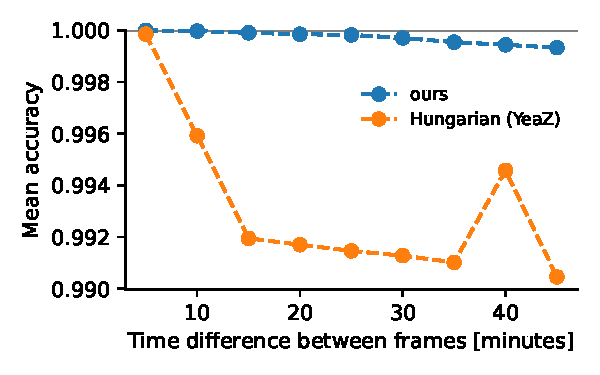
\includegraphics[width=\linewidth]{figures/timediff_mean_accuracy.pdf}
		\caption{Mean accuracy as a function of time difference between frames.}
		\label{fig:mean_acc}
	\end{figure}

	\subsection{Python environment}

		Training was performed using the following PyTorch ecosystem,
		\begin{verbatim}
			pytorch-lightning       1.7.5
			torch                   1.12.1
			torch-cluster           1.6.0
			torch-geometric         2.1.0.post1
			torch-scatter           2.0.9
			torch-sparse            0.6.15
			torch-spline-conv       1.2.1
			torchmetrics            0.10.0
		\end{verbatim}
		and data processing using the following Python scientific packages.
		\begin{verbatim}
			opencv-python           4.5.5.64
			numpy                   1.21.5
			scipy                   1.7.3
			pandas                  1.3.5
		\end{verbatim}

		Refer to \texttt{conda\_env.yaml} on the Github repository for full details.

	\subsection{Details of the microscope}
		
		Images were recorded using a Nikon Ti2-E microscope equipped with a 60x objective and a Hamamatsu Orca-Flash 4.0 camera.
		The microscope was operated using NIS-Elements software and the objective's axial position was controlled by Nikon
		Perfect Focus System. Images were taken every 5 min, with 100 ms exposure time for the the brightfield, GFP and mCherry
		channel.

	\subsection{Details of the strain}

		We used a W303-derived budding yeast strain with the following genotype: MATa ADE2 MYO1::MYO1-GFP::kanMX, 
		HTB2::HTB2-mCherry::HIS5.

	\subsection{Details of media and microfluidics chip used for growth}

		Cells were grown in CellASIC ONIX plate for haploid yeast cells in media controlled by the ONIX2 microfluidics system
		(Merck, Germany). We used standard synthetic complete medium with 2\% (v/v) glucose.

\end{document}
